\documentclass[11pt,t]{beamer}
\usepackage{graphicx}
\setbeameroption{hide notes}
\setbeamertemplate{note page}[plain]


\usetheme{default}
\beamertemplatenavigationsymbolsempty
\hypersetup{pdfpagemode=UseNone} % don't show bookmarks on initial view

\usepackage{physics}
\usepackage{xcolor}

% font
\usepackage{fontspec}
%\setsansfont{TeX Gyre Heros}
%\setbeamerfont{note page}{family*=pplx,size=\footnotesize} % Palatino for notes

\definecolor{offwhite}{RGB}{249,242,215}
\definecolor{foreground}{RGB}{255,255,255}
\definecolor{background}{RGB}{24,24,24}
\definecolor{title}{RGB}{107,174,214}
\definecolor{gray}{RGB}{155,155,155}
\definecolor{subtitle}{RGB}{102,255,204}
\definecolor{hilight}{RGB}{102,255,204}
\definecolor{vhilight}{RGB}{255,111,207}
\definecolor{lolight}{RGB}{155,155,155}

% use those colors
\setbeamercolor{titlelike}{fg=title}
\setbeamercolor{subtitle}{fg=subtitle}
\setbeamercolor{institute}{fg=gray}
\setbeamercolor{normal text}{fg=foreground,bg=background}
\setbeamercolor{item}{fg=foreground} % color of bullets
\setbeamercolor{subitem}{fg=gray}
\setbeamercolor{itemize/enumerate subbody}{fg=gray}
\setbeamertemplate{itemize subitem}{{\textendash}}
\setbeamerfont{itemize/enumerate subbody}{size=\footnotesize}
\setbeamerfont{itemize/enumerate subitem}{size=\footnotesize}

% page number
\setbeamertemplate{footline}{%
    \raisebox{5pt}{\makebox[\paperwidth]{\hfill\makebox[20pt]{\color{gray}
          \scriptsize\insertframenumber}}}\hspace*{5pt}}

% add a bit of space at the top of the notes page
\addtobeamertemplate{note page}{\setlength{\parskip}{12pt}}

% title info
\title{Avances de la tesina}
%\subtitle{A researcher's perspective}
\author{Isaí E. Dávila Cuba}
%\institute{\href{https://www.biostat.wisc.edu}{Biostatistics \& Medical Informatics} \\[2pt] \href{http://www.wisc.edu}{University of Wisconsin{\textendash}Madison}}
\date{28 de junio del 2021}

% Todos mis shorcuts para escribir más rápido.

\DeclareMathOperator{\Ran}{Ran}
\DeclareMathOperator{\Ker}{Ker}
\DeclareMathOperator{\im}{Im}



\newcommand{\imp}{\implies}			% Simbolo de implicacion
\newcommand{\supr}[1]{\underset{#1}{\sup}}
\newcommand{\mbf}[1]{\mathbf{#1}}     % Negrita en modo matemático
\newcommand{\lra}{\leftrightarrow}     % Flecha derecha e izquierda
\newcommand{\h}{\hat}             % hat para operadores
\newcommand{\red}[1]{\color{red}{#1}}
\newcommand{\green}[1]{\color{green}{#1}}
\newcommand{\blue}[1]{\color{blue}{#1}}
\newcommand{\pr}{\partial}      % Abreviacion para \partial
\newcommand{\cd}{\cdot}           % \cdot
\newcommand{\cds}{\cdots}           % \cdots
\newcommand{\inceq}{\subseteq}    % incluido e igual
\newcommand{\vc}[1]{\vec{#1}}     % vector
\newcommand{\dg}{^\dagger}
\newcommand{\conj}[1]{#1^*}       % conjugado
\newcommand{\pescalar}[2]{#1\cd #2}    % Producto escalar
\newcommand{\f}[2]{\frac{#1}{#2}}           % Short version for \frac
\newcommand{\dott}[1]{\overset{\cdot\cdot}{#1}} % Doble Punto encima (dt)
\newcommand{\nab}{\nabla}     % Shortcut for nabla
%\newcommand{\eval}{\big\rvert}  % Raya vertical para indicar evaluación
%\newcommand{\deg}[1]{#1^{\circ}}    % Grados
\newcommand{\la}{\leftarrow}        % Leftarrow
\newcommand{\mc}[1]{\mathcal{#1}}      % Tipografia caligrafia
\newcommand{\mf}[1]{\mathfrak{#1}}      % Tipografia frakture (gótico)
\newcommand{\ms}[1]{\mathscr{#1}}		% Cursiva
\newcommand{\tf}{\therefore }			% Los tres puntitos en triangulo
\newcommand{\sder}[2]{\frac{d #1}{d #2}} % Derivada simple de #1 respecto a #2
\newcommand{\der}[3]{\frac{d^{#1}#2}{d #3^{#1}}}  % Derivada n-sima de #1 respecto a #2
\newcommand{\sparc}[2]{\frac{\partial #1}{\partial #2}} %Derivadas parciales
\newcommand{\parc}[3]{\frac{\partial^{#1}#2}{\partial #3^{#1}}} %Derivada parcial n-esima respecto de #3
\newcommand{\m}[1]{\mathbb{#1}}	% Hace una letra R --> \mathbb{R}
\newcommand{\inc}{\subset}   % Incluido
\newcommand{\ndvec}[2]{(#1_1,#1_2,\ldots,#1_{#2})} %Crea un vector #2-dimensional con nombre #1
\newcommand{\ci}{\imath}		% Unidad imaginaria
\newcommand{\ptodo}{\forall}	% Para todo simbolo
\newcommand{\me}[1]{#1\m Z}		% Multiplos enteros de #1: #1Z.
\newcommand{\tq}{\mid}			% Simbolo para tal que...
\newcommand{\pp}[1]{#1^{\prime\prime}\mkern-1.2mu} %#1´´
\newcommand{\e}[1]{e^{#1}}		% Exponencial de #1
\newcommand{\om}{\omega}			% Shortcut para omega
\newcommand{\Om}{\Omega}			% Shortcut para Omega
\newcommand{\lam}{\lambda}          % Lambda
\newcommand{\Lam}{\Lambda}         % Lambda mayuscula
\newcommand{\al}{\alpha}          % alpha
\newcommand{\be}{\beta}           % beta
\newcommand{\gm}{\gamma}         % gamma
\newcommand{\Gm}{\Gamma}          % Gamma
\newcommand{\del}{\delta}         % Delta
\newcommand{\sg}{\sigma}          % Sigma
\newcommand{\Del}{\Delta}
\newcommand{\rel}{\sim}
\newcommand{\uvec}[1]{\bm{\hat{\mathbf{#1}}}}   % Vector unitario
\newcommand{\vct}[1]{\vec{\mathbf{#1}}}
\newcommand{\ra}{\rightarrow}
\newcommand{\eps}{\epsilon}
\newcommand{\ex}{\exists}
\newcommand{\bp}[1]{\left(#1\right)}
\newcommand{\bb}[1]{\left[#1\right]}
\newcommand{\bl}[1]{\left\{#1\right\}}
\newcommand{\deld}[1]{\delta^{(3)}(#1)}      % Delta de Dirac en 3d
\newcommand{\ddrc}[2]{\delta^{(#1)}(#2)}      % Delta de Dirac en Nd
\newcommand{\lrpr}{\overset{\lra}{\pr}}		% left right partial
\newcommand{\slashd}{\kern-0.5em\raise0.22ex\hbox{/}}
\newcommand{\barra}[1]{\cancel{#1}}


\usepackage[framemethod=TikZ]{mdframed}
\newtheorem{teora}{Teorema}
\mdfdefinestyle{myestyth}{roundcorner=5pt,skipabove=1pt,skipbelow=0pt,backgroundcolor=background,outerlinecolor=offwhite}\newcommand{\teo}[2]{
	\begin{mdframed}[style=myestyth]
	\begin{teora}[\textbf{#1}]		% Comienza el entorno teorema
	#2
	\end{teora}
	\end{mdframed}
	}


\usepackage[english]{babel}
\usepackage[utf8x]{inputenc}


\usepackage{amsthm, amssymb, amsfonts, amsmath}
\usepackage{graphicx}
\usepackage{tikz}
\usetikzlibrary{calc,shapes}
% \usepackage{enumitem}
\usepackage{mathtools}
\usepackage{mathrsfs}
%\usepackage{tikz-cd}

\newcommand{\subt}[1]{{\footnotesize \color{subtitle} {#1}}}

\begin{document}

\begin{frame}
  \titlepage
\end{frame}

\begin{frame}{Modelo abeliano de Higgs}

$\phi:\m R^{2+1}\ra\m C$ es un campo escalar complejo acoplado al campo electromagnético mediante acoplamiento mínimo
\begin{align}
    \mc L = -\f 14 F_{\mu\nu}F^{\mu\nu}+\f 12D_\mu\phi\overline{D^\mu\phi}-\f{\lambda}8(1-|\phi|^2)^2
\end{align}
Ecuaciones de Euler-Lagrange
\begin{align}
    D_\mu D^\mu\phi+\f{\lambda}2(1-|\phi|^2)\phi &= 0\\
    \pr_\mu F^{\mu\nu} &= J^\nu
\end{align}
donde $J^\mu=\f{i}2(\bar\phi D^\mu\phi-\phi\overline{D^\mu\phi})$.
Buscamos soluciones estáticas y con energía finita. Definimos el funcional de energía $V_\lambda$
\begin{align}
    V_\lambda = \f 12\int_{\m R^2}\bp{B^2+D_i\phi\overline{D_i\phi}+\f\lambda 4(1-|\phi|^2)^2}d^2x
\end{align}

\end{frame}

\begin{frame}

Condiciones de contorno en el infinito ($|\vct x|\ra\infty$) para que $V_\lambda$ sea finita
\begin{align}
    |\phi|&\ra 1\\
    B&\ra 0\\
    D_i\phi &\ra 0
\end{align}
Estas condiciones de contorno y simetría permiten escribir el \emph{ansatz} de Nielsen-Olesen o vortices radiales
\begin{align}
    \phi(\rho,\theta) &= f_N(\rho)e^{iN\theta}\\
    A_\theta(\rho,\theta) &= N\al_N(\rho)\\
    A_\rho &= 0
\end{align}
\begin{align}
    \f{d^2f_N}{d\rho^2}+\f{1}{\rho}\f{df_N}{d\rho}-\f{1}{\rho^2}(N-\al_N)^2 f_N+\f{\lambda}2(1-f_N^2)f_N &=0\\
    \f{d^2\al_N}{d\rho^2}-\f{1}\rho\f{d\al_N}{d\rho}+(N-\al_N)f_N^2 &= 0
\end{align}
    
\end{frame}

\begin{frame}{Soluciones numéricas}

\begin{columns}
\column{0.5\textwidth}
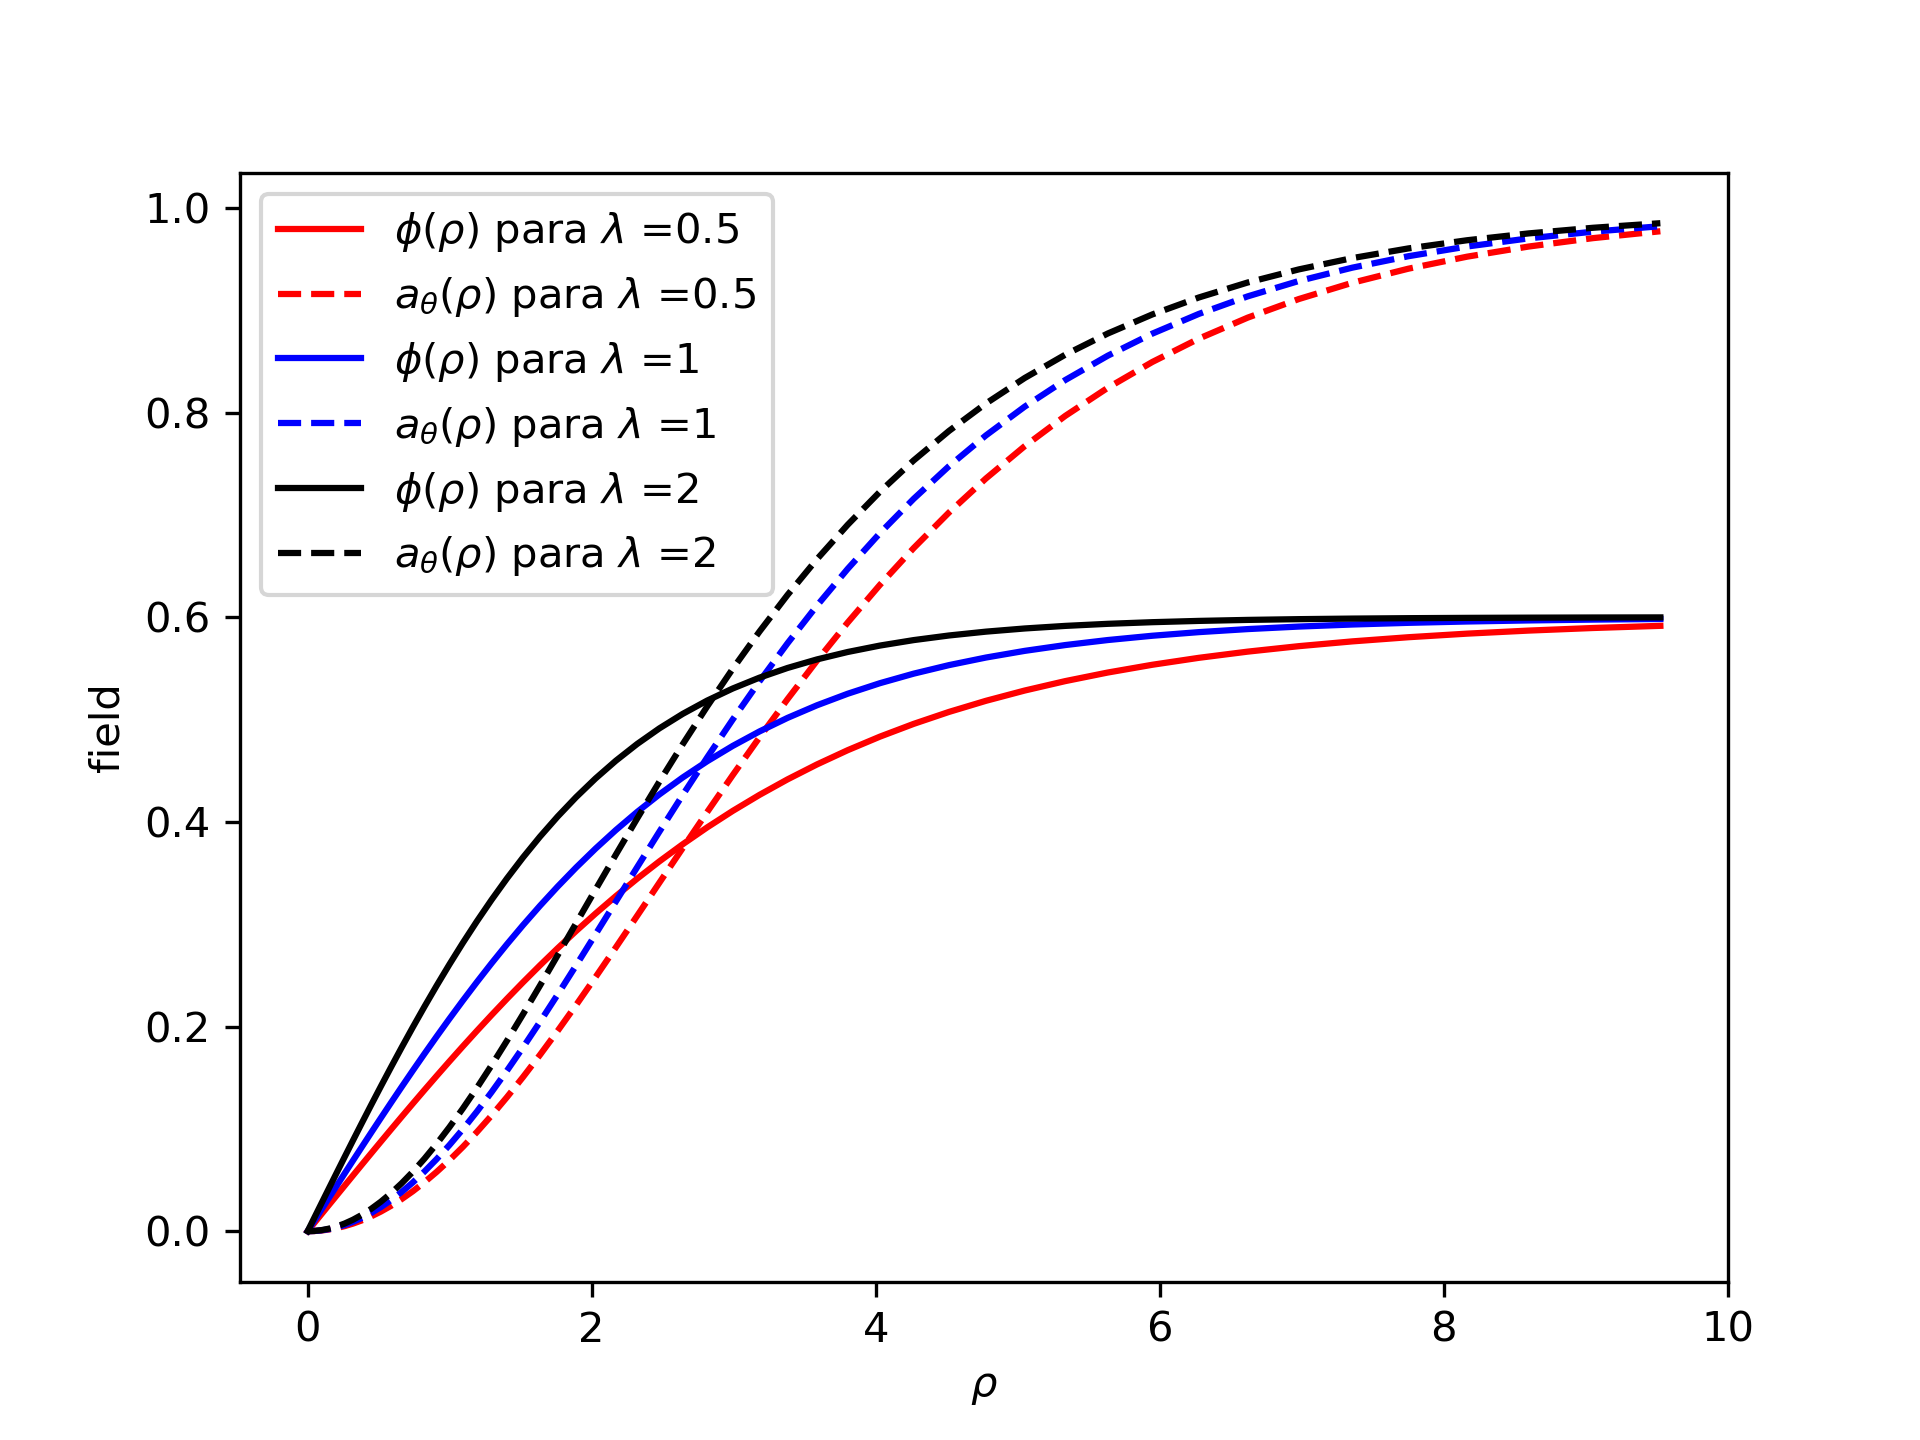
\includegraphics[width=0.9\textwidth]{fields.png}\\
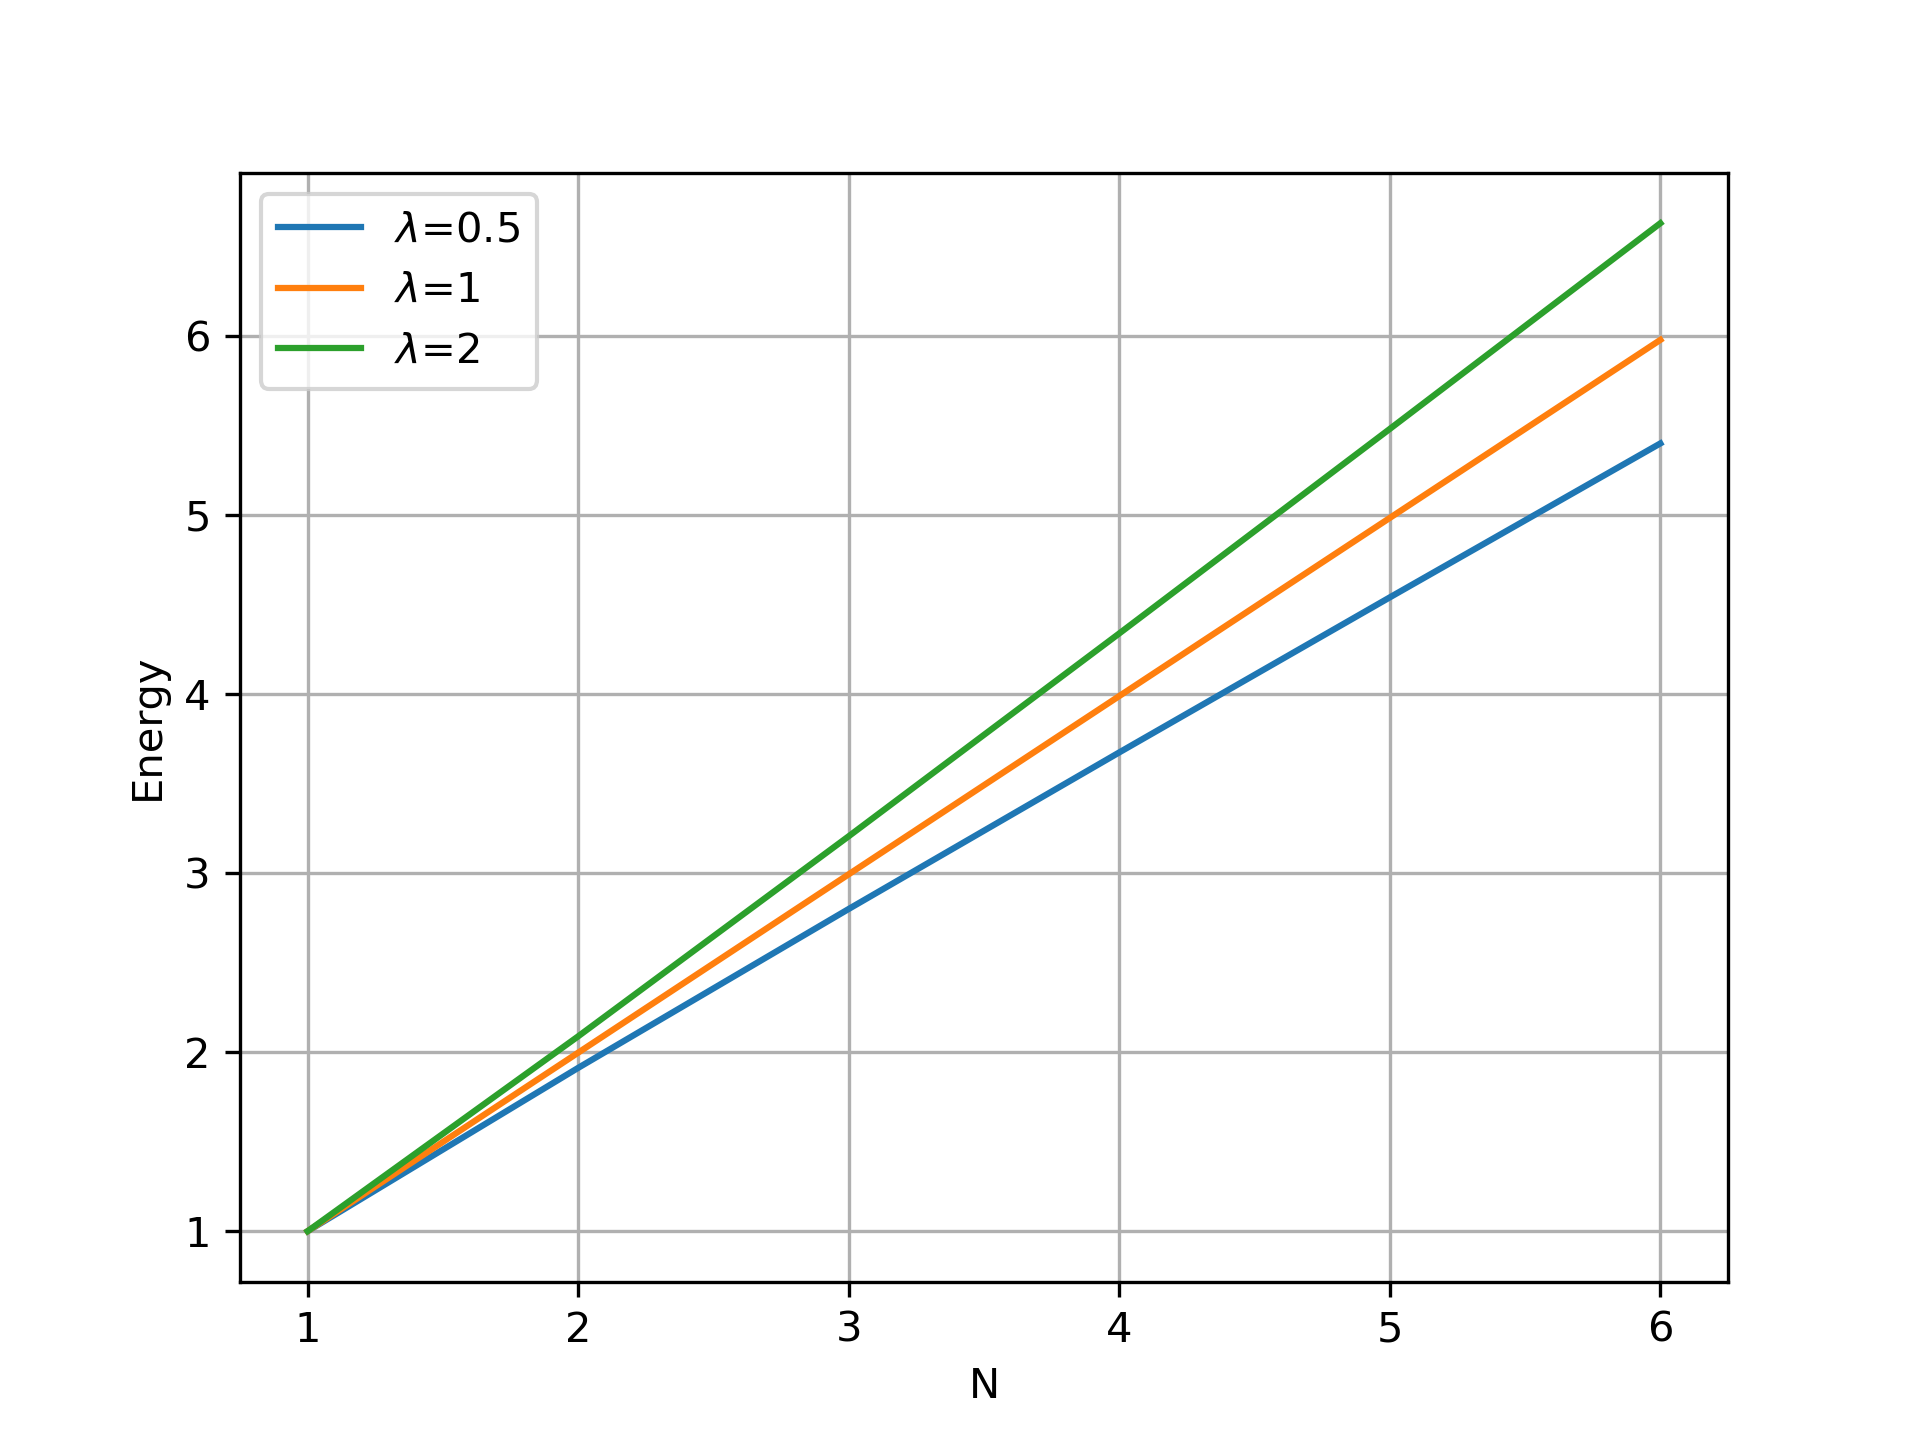
\includegraphics[width=0.9\textwidth]{Energy.png}
\column{0.5\textwidth}
Gráficas de los campos y de la energía obtenidos numéricamente en Python.
\end{columns}
    
\end{frame}


\begin{frame}{Vórtices críticos}

Completamos cuadrados a la Bogomolny y obtenemos un límite inferior para el funcional de energía para $\lambda=1$.
 \begin{align}
     V_{\lambda=1} = \f 12\int_{\m R^2}\bb{\bp{B-\f{1}2(1-|\phi|^2)}^2+|D_1\phi+iD_2\phi|^2}d^2x+ \pi N 
 \end{align}
 \begin{align}
 V_{\lambda=1}\geq \pi N
 \end{align}
El límite se satura si $\phi$ satisface las ecuaciones de Bogomolny
 \begin{align}
     \left\{\begin{array}{c}
          D_1\phi+iD_2\phi = 0  \\
          B = \f 12(1-|\phi|^2)
     \end{array}\right.
 \end{align}

\end{frame}

\begin{frame}

La primera ecuación se puede escribir como una condición de analiticidad análoga a las ecuaciones de Cauchy-Riemann
\begin{align}
D_{\bar z}\phi =0
\end{align}
Escribiendo $f=e^{-\om}\phi$, se puede mostrar que $\pr_{\bar z}f=0$ si $\pr_{\bar z}\om= i A_{\bar z}$. Por lo tanto, si podemos encontrar una solución para $\om$, la función $f$ es analítica. La solución está dada por la fórmula de Cauchy-Pompeiu para $A_{\bar z}=0$ en el borde de $D$.
\begin{align}
\om(z) = -\f{1}{2\pi i}\iint_D \f{iA_{\bar z}}{z-u}d\bar u\wedge du
\end{align}
Como $f$ es analítica, tiene ceros aislados y cerca de los ceros
\begin{align}
f\sim c_j(z-z_j)^{n_j}, \ \ n_j\in\m N
\end{align}
Estos ceros corresponden a los ceros de $\phi$ también, pues $e^{-\om}\neq 0$. $z_j$ no son otra cosa que los centros de los vórtices donde $B=0$.

\end{frame}

\begin{frame}{Reducción a la ecuación de Taubes}

Una vez que se conoce una solución $\phi$, el campo de gauge queda determinado por
\begin{align}
    A_{z} = i\pr_{z}\log\bar\phi, \ \ A_{\overline z} = -i\pr_{\overline z}\log\phi
\end{align}
Escribiendo $\phi=e^{u}$ e insertando (19) en $B = 2i(\pr_z A_{\overline z}-\pr_{\overline z}A_z$ y finalmente reemplazando todo en la segunda ecuación de Bogomolny, llegamos a la ecuación de Taubes \cite{noauthor_jaffe_nodate}
\begin{align}
\Delta u-e^u+1=0
\end{align}

\teo{Teorema de Taubes}{Dado un entero $N\geq 0$ y un conjunto de puntos $\{z_i\}, i=1,2,\cds N$ en el plano complejo $\m C$, existe una solución de las ecuaciones de Bogomolny que es única a menos de una transformación de gauge}

\end{frame}

\begin{frame}{Vortices en superficies de Riemann}

No se conoce soluciones explícita para la ecuación de Taubes en el plano hasta la fecha. Pueden existir soluciones explícitas en espacios curvos. Cambiemos la métrica plana por
\begin{align}
ds_0^2 = \Om_0((dx^1)^2+(dx^2)^2)=\Om_0 dzd\bar z
\end{align}
donde $\Om_0$ es un factor conforme y $z=x+iy$. Esta métrica define una superficie de Riemann $M_0$. Podemos considerar la ecuación de Taubes definida en $M_0$
\begin{align}
-\f 1{\Om_0}\Delta u+e^u-1 =0
\end{align}

\end{frame}

\begin{frame}{Más ecuaciones de vórtices}

Consideremos $C_0$ y $C$ dos constantes. Generalizamos la ecuación de Taubes en $M_0$ de la siguiente forma
\begin{align}
-\f{1}{\Om_0}\Delta u-Ce^u+C_0 =0
\end{align}
Las constantes pueden tomar cualquier valor, sin embargo, se tienen tres valores estándar $-1,0,1$. Por lo tanto, nueve ecuaciones vorticiales. Sólo cinco son físicamente viables. [Manton]

\begin{table}[ht]
    \centering
    \begin{tabular}{l|c|c}
        Vórtices & $C_0$ & C \\ \hline
        Vórtices hiperbólicos (Taubes) & -1 & -1\\
        Vórtices de Popov & 0 & 1\\
        Vórtices de Jackiw-Pi & 1 & 1\\
        Vórtices de Bradlow & -1 & 0\\
        Vórtices de Ambjorn-Olesen & -1 & 1\\ \hline
    \end{tabular}
    \label{tab:vortex}
\end{table}

\end{frame}

\begin{frame}

Vórtices hiperbólicos fueron obtenidos por primera vez por Witten [Witten77] en términos de una función analítica $f:\m H^2\ra\m H^2$
\begin{align}
\phi = \f{1-|z|^2}{1-|f|^2}\f{df}{dz}
\end{align}
En el modelo del disco de Poincaré,
\begin{align}
f(z) = \prod_{n=1}^{N+1}\f{z-a_n}{1-\bar{a_n}z}
\end{align}
donde $|a_n|<1$.

En particular $f(z)=z^{N+1}$. En este caso, hay $N$ vórtices coincidentes en el origen.

\end{frame}

\begin{frame}{Generalizando }
En [Baptista]\cite{baptista_vortices_2013} se sugiere la siguiente métrica
\begin{align}
ds^2 = |\phi|^2 ds_0^2 = e^{u}ds_0^2
\end{align}  
La métrica original reescaleada confomemente con el cuadrado del campo de Higgs. Métrica de Baptista no es regular pues se hace cero en los centros de los vórtices $\phi=0$. Definimos nuevo factor conforme $\Om=e^u\Om_0$. Las curvaturas de las superficies que estas métricas definen están relacionadas por la ecuación de Baptista
\begin{align}
(K_0-C_0)\Om_0=(K-C)\Om
\end{align}

\end{frame}

\begin{frame}{Vortices integrables}
Cuando la curvatura de $M_0$, $K_0$, es contante y toma un valor específico de acuerdo a su ecuación de vórtice, decimos que tal ecuación es integrable. Este valor específico es aquel que satisface la ecuación de Baptista, $K_0=C_0$. Entonces, la métrica de Baptista tiene curvatura constante $K=C$, excepto en las singularidades.

Como, $M_0$ y $M$ tienen curvatura constante, sus factores conforme $\Om_0$ y $\Om$ deben satisfacer la ecuación de Liouville
\begin{align}
\Delta\log\Om_0 &= -2K_0\Om_0\\
\Delta\log\Om &= -2K\Om
\end{align}
Solución general es conocida
\begin{align}
\Om &= \f{4}{(1+C|f(z)|^2)^2}\left|\f{df}{dz}\right|^2\\
\Om_0 &= \f{4}{(1+C_0|z|^2)^2}
\end{align}

\end{frame}

\begin{frame}
Entonces, solución general es
\begin{align}
|\phi|^2 = \f{\Om}{\Om_0} = \f{(1+C_0|z|^2)^2}{(1+C|f(z)|^2)^2}\left|\f{df}{dz}\right|^2
\end{align}
Podemos elegir,
\begin{align}
\phi = \f{1+C_0|z|^2}{1+C|f(z)|^2}\f{df}{dz}
\end{align}
Los puntos donde $\f{df}{dz}=0$ son los centros de los vórtices $\phi=0$.
\end{frame}

\begin{frame}{Ecuaciones de Bogomolny y Supersimetría}
\subt{Extensión $N=1$ del modelo abeliano de Higgs en $2+1$}

En [Edelstein94] propusieron la siguiente extensión supersimétrica de la ección del modelo abeliano de Higgs
\begin{align*}
L_{N=1} = \int d^2\theta\left\{\f 12 W^\al W_\al-\f 14(\mc D^\al+ie\Gamma^\al)\Phi\dg(\mc D_\al-ie\Gamma_\al)\Phi-\right.\\ 
\left.\f 14\mc D^\al S\mc D_\al S+\sqrt{2\lambda}S\Phi\dg\Phi+\eta S\right\}
\end{align*}
donde $\mc D^\al$ es la superderivada covariante, $\Gm^\al$ es el supercampo vectorial, $W^\al$ es el supercampo electromagnético, $\Phi$ es un supercampo escalar complejo y $S$ un supercampo escalar real.
\begin{align}
\Phi(x;\theta) &= \phi(x)+\bar\theta\psi(x)-\f 12\bar\theta\theta F(x)\\
\Gm_\al(x;\theta) &= iA_\mu(x)(\gm^\mu\theta)_\al-\bar\theta\theta\rho_\al(x)\\
S(x;\theta) &= N(x)+\bar\theta\chi(x)-\f 12\bar\theta\theta D(x)
\end{align}
\end{frame}

\begin{frame}
\begin{align*}
L_{N=1} = -\f 14 F^{\mu\nu}F_{\mu\nu}+\f 12\pr^\mu N\pr_\mu N+\f 12(D^\mu\phi)\dg D_\mu\phi-4\lambda N^2|\phi|^2\\
-\lambda(|\phi|^2-\phi_0^2)^2+\f i2\bar\rho\gm^\mu\pr_\mu\rho+\f i2\bar\chi\gm^\mu\pr_\mu\chi+\f i2\bar\psi\gm^\mu D_\mu\psi-\sqrt{2\lambda}N\bar\psi\psi\\
+\f{ie}2(\bar\psi\rho\phi-\bar\rho\psi\phi\dg)-\sqrt{2\lambda}(\bar\psi\chi\phi+\bar\chi\psi\phi\dg)
\end{align*}
Es posible extender esta simetría $N=1$ a una simetría $N=2$ haciendo el parámetro infinitesimal $\eps$ complejo $\eps^c$, y juntando los fermiones reales en $\Sigma=\chi-i\rho$. Para esto debemos imponer una condición sobre la constante de acoplamiento. Esta es
\begin{align}
\lambda = \f{e^2}8
\end{align}
Esta es la condición obtenida para obtener las ecuaciones de Bogomolny de antes.
\end{frame}

\begin{frame}
La corriente de Noether asociada a la supersimetría se puede calcular y a partir de esta, obtener la carga conservada. Escrita como $\mc Q=\bar\eps^c Q+\bar Q\eps^c$, para eliminar la variable de Grassmann infinitesimal, se tiene que
\begin{align*}
Q = \int d^2x\left[\bp{-\f 12\eps^{\mu\nu\lambda}F_{\mu\nu}\gm_\lambda+i\gm^\mu\pr_\mu N-\f{e}2(|\phi|^2-v^2)}\gm^0\Sigma\right.\\
\left.\bp{i(\gm^\mu D_\mu\phi)\dg-\f{e}2N\phi\dg}\gm^0\psi\right]\\
\bar Q = \int d^2x\bar\Sigma\gm^0\left[\bp{-\f 12\eps^{\mu\nu\lambda}F_{\mu\nu}\gm_\lambda+i\gm^\mu\pr_\mu N-\f{e}2(|\phi|^2-v^2)}\right.\\
\left.\bar\psi\gm^0\bp{-i\gm^\mu D_\mu\phi-\f{e}2N\phi}\right]
\end{align*}
Para configuraciones estáticas y en el gauge $A_0=0$, las cargas satisfacen la siguiente relación de anticonmutación
\begin{align}
\{Q_\al,\bar Q^\be\}=2(\gm_0)^\be_\al P^0+\delta^\be_\al T
\end{align}

\end{frame}

\begin{frame}
Donde $P_0$ no es más que la energía
\begin{align}
P^0 = E = \int d^2x\bp{\f 14 F_{ij}^2+\f 12|D_i\phi|^2+\f{e^2}8(\phi_0^2-|\phi|^2)^2}
\end{align}
Y $T$ es la carga central
\begin{align}
T = e\phi_0^2\bp{\f{2\pi}e}N, \ \ N\in\m Z
\end{align}
Elevando al cuadrado la relación de conmutación se puede obtener un límite para la energía
\begin{align}
E\geq\f{|T|}2
\end{align}
No es más que el mismo inferior para la energía obtenido a la Bogomolny.
\end{frame}

\begin{frame}
Para obtener explícitamente las ecuaciones de Bogomolny a partir del álgebra supersimétrica, definamos
\begin{align}
Q_I &= \f{Q_++iQ_-}{\sqrt 2}\\
Q_{II} &= \f{\bar Q^++i\bar Q^-}{\sqrt 2}
\end{align}
donde $Q = (Q_+,Q_-)^T$ y $\bar Q=(\bar Q^+,\bar Q^-)$.

Un estado $\ket{B}$ que sature la desigualda de Bogomolny, necesariamente es aniquilado por las cargas, entonces, necesariamente
\begin{align}
(Q_I\pm Q_{II})\ket{B} =0
\end{align}
\end{frame}

\begin{frame}
Si esto ocurre entonces
\begin{align}
\f 12\eps_{ij}F^{ij} &= \f{e}2(\phi_0^2-|\phi|^2)\\
D_i\phi+iD_2\phi &=0
\end{align}
Estas son las ecuaciones de Bogomolny.
\end{frame}

\begin{frame}{Modelos abelainos de Higgs modificados}

Podemos modificar el lagrangiano del modelo abeliano de Higgs admitiendo términos cinéticos no estándar [Sourrouille]
\begin{align}
L = \int d^2x\bp{-\f 14F_{\mu\nu}F^{\mu\nu}+\textcolor{red}{\om(\phi)}|D_\mu\phi|^2-V(\phi)}
\end{align}
o también [Contatto],
\begin{align}
L = \int d^2x\textcolor{blue}{\Om}\bp{-\f {\textcolor{red}{G(|\phi|)^2}}4F_{\mu\nu}F^{\mu\nu}+|D_\mu\phi|^2-V(\phi)}
\end{align}
Podemos contreñir la forma de estas funciones con condiciones de contorno en el infinito o de acuerdo a la forma de $V(\phi)$.

\end{frame}

\begin{frame}
Por ejemplo si elegimos $V(\phi)=\f{\lambda}4(1-|\phi|^{2(n+1)})$, necesariamente
\begin{align}
\om(\phi) = \sqrt{\lambda}(n+1)|\phi|^{2n}
\end{align}
para obtener un análogo al límite de Bogomolny. En este caso, $E\geq 2\pi N\sqrt\lambda$. El límite se satura cuando
\begin{align}
B = -\f{\sqrt\lambda}2(1-|\phi|^{2(n+1)})\\
\phi^n(D_1+iD_2)\phi = 0
\end{align}
\end{frame}

\begin{frame}{Referencias}
\bibliography{biblio}
\end{frame}


\end{document}
